\documentclass{article}
\usepackage{amsmath}
\usepackage{bm}
\usepackage[capposition=top]{floatrow}
\usepackage{float}
\usepackage{amssymb}
\usepackage{amscd}
\usepackage{csquotes}
\usepackage{biblatex}
\addbibresource{bibliography.bib}

\usepackage{graphicx}
\graphicspath{ {./images/} }

\usepackage{amsthm}
\theoremstyle{definition}
\newtheorem{definition}{Definition}[section]
\newtheorem{theorem}{Theorem}[section]
\theoremstyle{definition}


\title{Knowledge Distillation in Matrix Product State Tensor Networks}
\author{Dereck Piché}
\date{\today}


\begin{document}
\maketitle


\section{Introduction}



\section{Knowledge Distillation}
Knowledge Distillation is a machine learning practice which involves
taking a trained model and using its parameters to train another one.
The already trained model is referred to as the "teacher", and 
the model in which his "knowledge" is to be distilled is referred to as
the "student". While this is a relatively novel technique, there are 
already several distinct approaches introduced by researchers.
In this project, we used two of these approaches. Our inspiration for the distillation 
methodology was found in a a 2021 survey which resumed the emerging 
practice \cite{Gou_2021}.

\subsection{Response-Based Knowledge Distillation}
The first approach we used was \emph{Response-Based Knowledge Distillation}. The idea of this approach is to stimulate the teacher and the student with some input and to try to minimise a certain loss function with respect to the teacher and student outputs. For classification tasks, it is recommended to use the Kullback-Leibler divergence as our loss function. 
\begin{equation}
    KL(P, Q) = \frac{1}{n} \sum_i^n Q \frac{log_e(Q)}{log_e(P)}
\end{equation}
Here, $Q$ is the distribution we are aiming for and $P$ is the one we have.

The reason is quite simple. Since it's a classification task, it is expected that the teacher and student will, given an input, return a probability distribution for each class. As is currently common, we used the softmax function on the logits of the student and the teacher in order to obtain probability distributions corresponding to the classes. 

\begin{equation}
    softmax(v_i) = \frac{e^{v_i}}{\sum_{j}{e^{v_j}}}
\end{equation}

Now, it would be logical to use a function aimed at measuring the difference between two probability distributions as our loss function. This is exactly what the Kullback-Leibler divergence is for.

\subsection{Layer-based approach}
The survey on Knowledge Distillation coined the term {\it Layer-based approach}.
Deep learning models work in layers of feature maps. It is hypothesized that
these different layers represent different layers of abstraction in the internal
representation of their input. If we use the Response-Based approach, it could prove difficult for gradient descent optimization to find these useful representation without a bit of help. This layer-based approach, as you might have guessed, aims to do precisely that. If our student model has some form of composition, we can train the parts separately. Thus, if an intermediate layer of the teacher $l$ were particularly useful, we could train a certain part of the student on the layer $l$ before proceding with the Response-Based approach.



\section{Tensor Networks}
Tensor Networks are mathematical objects which were created by physicists in order to help with the modelisation of quantum phenomena.
In 2017, researchers form the Flatiron institutes had the brilliant idea of using these networks as machine learning models \cite{stoudenmire2017supervised}. That is, to make them learn function in a supervised fashion. In order to make this report as self-contained as possible, we decided to provide a short explanation of what they are. Some confusion can be avoided by mentionning that the expression \emph{Tensor Networks} refers, in the scientific community, to both a series of methods and a notational system.

\subsection{Tensors}
Before explaining the methods and the notational system, we shall disambiguate the meaning of the word \enquote{tensor}. In physics, tensors are often paired with transformation properties. 
However, in this report (and very often in the context of machine learning), we use the word \enquote{tensor} to refer to mathematical arrays of arbitrary dimensions denoted by indices. Here, the number of indices is called the \enquote{order} of the tensor, meaning that vectors are simply tensors of order $1$ and matrices tensors of order $2$. An exemple of a tensor of higher order would be $T_{i_1,i_2,i_3,i_4}$. This tensor is of order $4$.

\subsection{Contraction}
At the heart of tensor networks is the {\it contraction} operation.
Tensor Networks are used to compute a larger network by "contracting" several
smaller tensors over chosen indices. A "contraction" is simply an operation 
where we sum over indices. For example, the contraction of $A_{ijk}$ and 
$B_{ijk}$ on index $j$ will produce the tensor $C_{ik} = \sum_{j} A_{ijk} B_{ijk}$.
Evidently, the two indices present in a contraction must be of the same size.

\subsection{Tensor Networks as a graphical system of notation}
The main motivation behind the creation of Tensor Networks is to compute or approximate large tensors by {\it contracting} several smaller tensors over chosen indices. Our visual representation of tensors as a block of numbers stops at order $3$. 
This is all well and good until our conventional summation notation begins overclocking our poor brains. 
So, in order to make the manipulation of these network of tensors, mathematicians created a notational system. 
Tensors are represented as nodes where each vertex connected to the node represents one of the tensor's indices. 
If a vertex connects two nodes, it means that the indices shall be contracted in order to produce the post-contraction tensor. 
It should be evident that by the definitions above, no node (tensor) is completely isolated in a tensor network, as it would be completely purposeless. 
The shape of the post-contraction tensor can be easily visually identified, since it is found in the unconnected vertices.
A simple tensor network can be found in figure \ref{fig:tensor_net}.
Let's translate this Tensor Network with the summation notation. First, we see that the result of the contractions of the smaller tensors $A$, $B$ and $C$ over their connected indices shall result in a tensor $T_{i, j, k}$, because $i$, $j$, and $k$ and the only indices that are not contracted. Since the other that the indices $l$, $m$ and $n$ are contracted, we will need to sum of them. Thus the tensor represented by the graphic is
\[ 
    T_{i, j, k} = \sum_{l, m, n} A_{j, l, m} B_{i, l, n} C_{m, n, k}
\]

\begin{figure}[hbt!]
    \centering
    \caption{A Very Simple Tensor Network Illustrating the notation.}
    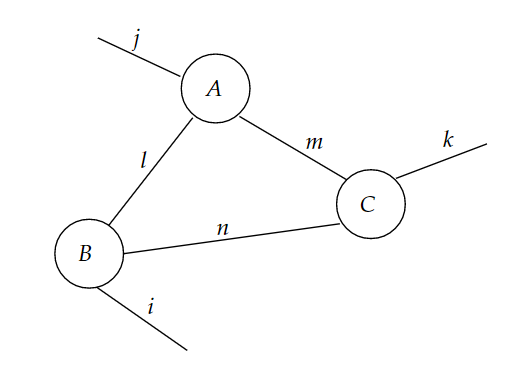
\includegraphics[width=0.8\textwidth]{images/2023-04-21-16-44-53.png}
    \label{fig:tensor_net}
\end{figure}

\subsection{Tensor Network Methods}
The term {\it Tensor Network Methods} is used to refer to, you guessed it, the methods.
There are several architectures of Tensor Networks that are frequently used, such as the {\it Matrix Product State (MPS)}, the \emph{Matrix Product Operator}, the \emph{MERA}, the \emph{Hierchical Tucker}, etc. As the title of this report indicates, 
There are many ways of transforming a Tensor into a contraction of smallers tensors. 
With time, some particular ways became popular for their properties. 
Some are faster to compute, some are clearer, some are easier to train in a machine learning context. 
One of these recurring architectures, the Matrix Product State, is at the core of this report.
Not only is there multiple valid ways of setting up the network for contractions, there are also different ways of performing the contraction.
In Tensor Networks, the order of contraction affects the computationnal complexity of the whole process!
All of these kinds of concepts are referred to by the expression \emph{Tensor Network Methods}. 

\section{Creating the function we will approximate}
In this report, we used the MPS tensor network to approximate a particular parameterizable function.
{\bf Troughout this report, the parameterizable function we are approximating with the MPS will be denoted by $\Upsilon_{T}$. }
We found it clearer to explain the $\Upsilon_{T}$ function we are approximating before introducing the MPS tensor network, as we we shall be able to explain the MPS through its use.
Now, enough talking (or rather, writing?), let's create the $\Upsilon_{T}$ function!

\subsection{Generating a feature space by using the Kronecker Product}
Consider an input vector $\mathbf{x} \in R^d$. Let $\phi : R \to R^{d_{\phi}}$ be a function which creates a feature map vector $\phi(x)$ from its input $x$.  We shall form the vector $\Phi(\mathbf{x})$ by taking the Kronecker product of the feature map $\phi(x_i)$ of every element of the input vector $\mathbf{x}$.
\begin{equation}
    \Phi(\mathbf{x}) = \phi(x_1) \otimes  \phi(x_2) 
                \otimes (\dots) \phi(x_d)
\end{equation}
Here, the symbol $\otimes$ represents the Kronecker Product. The Kronecker Product is an extremely generalisable operation that can be applied to a pair of tensors of arbitrary order. In this project, we use the Kronecker Product exclusively on vectors. Here is a simple example that illustrates what the kronecker product does for simple vectors of integers.
\[
\begin{bmatrix}
    9 \\ 4
\end{bmatrix}
\otimes
\begin{bmatrix}
    6 \\ 8
\end{bmatrix}
\otimes
\begin{bmatrix}
    7 \\ 3
\end{bmatrix}
=
\begin{bmatrix}
    54 \\ 72 \\ 24 \\ 32
\end{bmatrix}
\otimes
\begin{bmatrix}
    7 \\ 3
\end{bmatrix}
=
\begin{bmatrix}
    378 \\ 162\\ 504 \\216\\ 168\\ 72\\ 224\\ 96
\end{bmatrix}
\]
The element $i$ of the first operand vector becomes itself multiplied by the second operand vector. Here's a slightly more abstract example:
\[
    \begin{bmatrix}
        v_1 \\ v_2
    \end{bmatrix}
    \otimes
    \begin{bmatrix}
        u_1 \\ u_2
    \end{bmatrix}
    =
    \begin{bmatrix}
        u_1 v_1 \\ u_2 v_1 \\ u_1v_2 \\ u_2v_2
    \end{bmatrix}
\]
Thus, if we perform a Kronecker Product on $n$ vectors, it will produce a vector such that every of its element is a multiplication of $n$ elements, each one from a different vector. We can thus interpret $\Phi(\mathbf{x})$ as being a feature space vector which \emph{captures the multiplicative interaction of the elements of the $\phi(x_i)$ feature maps}. Here's a visual and intuitive way to think about the Kronecker Product applied to a set of vectors. Suppose we have the set of vectors and that we draw a square an element of each one

\[
    \begin{bmatrix}
        \boxed{9} \\ 4
    \end{bmatrix},
    \begin{bmatrix}
        6 \\ \boxed{8} \\ 5
    \end{bmatrix},
    \begin{bmatrix}
        \boxed{7} \\ 3
    \end{bmatrix}
\]
Then the product of these elements,  $9\times8\times7=504$, will find itself in the vector $v=
    \begin{bmatrix}
        9 \\ 4
    \end{bmatrix}
    \otimes
    \begin{bmatrix}
        6 \\ 8 \\ 5
    \end{bmatrix}
    \otimes
    \begin{bmatrix}
        7 \\ 3
    \end{bmatrix}
$. This statement would have been true had we chosen any other combination of the elements of each vector to surround with a square. This is was what was meant when we said that the resulting vector captures the \emph{multiplicative interaction of the elements}.



\subsection{The multilinear feature map}
Now, which feature map $\phi$ shall we pick in order to construct $\Phi$?
Well, normally, this would be up to you, but in this project we deal with the particular feature map:
\begin{equation}
    \phi_{ml}(x) = 
    \begin{bmatrix}
        1 \\
        x
    \end{bmatrix}
\end{equation}
We call this particular feature map the \emph{multilinear feature map}.
Why do we call it that? Because, amazingly, when we use this feature map, the elements of $\Phi(\mathbf{x})$ form a basis space of the multilinear functions on the elements of the vector $\mathbf{x}$.
Understanding this statement without a bit of context and help is a tall order. Let's deconstruct it.
First, what is a multilinear function? A multilinear function is a multivariate function that is linear for every variable if all the other variables are considered as constants. For example, $f(x_1, x_2) = x_1 x_2$ is a multilinear function because $x_1 c_2$ and $c_1 x_2$ are both linear functions. However, $f(x_1, x_2) = x_1 x_2^2$ is not a multilinear function, because the function $f(x_1, x_2) = c_1 x_2^2$ is not linear. A full explanation of vector spaces is out of the scope of this report. You can think of the space of multilinear function as a vector space. Not very rigourously, we can say that this is the case because it is possible to describe any particular multilinear function by choosing the coefficients $c_i$ in this expression :
\[
    c_1 1 + c_2 x_1 + c_3 x_2 + c_4 x_3  + c_5 x_1 x_3 + c_6 x_1 x_2 + c_7 x_2 x_3 + c_8 x_1 x_2 x_3
\]
For example, if we want the function $f(x) = 3 + 4 x_2 x_3$, we simply need $c_1 = 3$, $c_7 = 4$ and the rest to be equal to $0$.

Let us show you a simple example to illustrate this.
\[
    \Phi(\begin{bmatrix}x_1 \\ x_2 \\ x_3 \end{bmatrix})
    =
    \phi_{ml}(x_1) \otimes \phi_{ml}(x_2) \otimes \phi_{ml}(x_3)
    =
\]
\[
\begin{bmatrix}
    1 \\ x_1
\end{bmatrix}
\otimes
\begin{bmatrix}
    1 \\ x_2
\end{bmatrix}
\otimes
\begin{bmatrix}
    1 \\ x_3
\end{bmatrix}
=
\begin{bmatrix}
    1 \\ x_1
\end{bmatrix}
\otimes
\begin{bmatrix}
    1 \\ x_3 \\ x_2 \\ x_2 x_3
\end{bmatrix}
=
\begin{bmatrix}
    1 \\ x_3 \\ x_2 \\ x_2 x_3 \\ x_1 \\ x_1 x_3 \\ x_1 x_2 \\ x_1 x_2 x_3
\end{bmatrix}
\]
Now, it should be clear that if we take the inner product of a vector $V$ and 
\[
    \langle V,  \Phi \left(\begin{bmatrix}x_1 \\ x_2 \\ x_3 \end{bmatrix}\right) \rangle
\]
which is equivalent to taking a linear combination of the elements of the vector, 
$\Phi(\begin{bmatrix}x_1 \\ x_2 \\ x_3 \end{bmatrix})$, we can express any multilinear function of the variables $x_1$, $x_2$ and $x_3$ by choosing the appropriate vector $V$.
\subsection{Linear Combinations}

When we introduced $\Upsilon_{T}$, we said it was a parameterizable function. However, as of yet, everything described about the function as been deterministic and fully specified. Thus, it is time to introduce the parameters. The parameters will be the coefficients of a linear map applied to the vector $\Phi(\mathbf{x})$. You might be asking yourself why go through all this? It has to do with expressivity. If we take the linear combinations of $\mathbf{x}$ directly, we will be limited to linear functions. However, in practice, many functions are fundamentally non-linear. They can't even be approximated well by linear functions. Thus, we project the initial vector $\mathbf{x}$ in a new non-linear space before applying the linear map. This is why we chose the $\phi_{ml}$. Multilinear functions are extremely expressive. Their limitations (as well as a way to bypass them) shall be discussed later in this report. \\ 


If we apply a dot product, we obtain an extremely expressive function.
\[
    V 
    \left(\phi_{ml}(x_1) \otimes \phi_{ml}(x_2)\otimes \dots \otimes \phi_{ml}(x_d) \right)
\]
where $V \in R^{2_d}$.
Now, here is the interesting part. Instead of doing this explicitely, we can reformulate the exact same model by using a contraction between a tensor $T$ and the feature map vectors : 
\[
    \sum_{i_1, i_2, \dots, i_d} T_{i_1, i_2, \dots, i_d}
    \left(
    \begin{bmatrix}
        1 \\ x_1
    \end{bmatrix}_{i_1}
    \cdot
    \begin{bmatrix}
        1 \\ x_2
    \end{bmatrix}_{i_2}
    \cdot
    (\dots)
    \cdot
    \begin{bmatrix}
        1 \\ x_d
    \end{bmatrix}_{i_e}
    \right)
\]
This creates a fonction $f: R^d \to R$. If instead we want a function that maps to $R_h$, we can add an index $h$ on the tensor $T$ such that it becomes $T^{h}_{i_1, i_2, \dots, i_d}$. At long last, we have all the ingredients to finally define the $\Upsilon_t :  R^d \to R^h$ function~:
\[
    \Upsilon_T(\mathbf{x}) =     \sum_{i_1, i_2, \dots, i_d} T^{h}_{i_1, i_2, \dots, i_d}
    \cdot
    \begin{bmatrix}
        1 \\ x_1
    \end{bmatrix}_{i_1}
    \cdot
    \begin{bmatrix}
        1 \\ x_2
    \end{bmatrix}_{i_2}
    \cdot
    (\dots)
    \cdot
    \begin{bmatrix}
        1 \\ x_d
    \end{bmatrix}_{i_d}
\]
You might be wondering why we didn't introduce the $Y_T$ function in this fashion right away. We simply thought that thinking about linear combinations of the elements given by the Kronecker Product gives a better intuition then the summation notation needed to describe the Tensor Network for the readers who are unacostumed to it. Now, we have function that is, theoretically, trainable by the use of supervised learning. We simply have to modify the tensor $T$, which represents the parameters of the model.

\section{The \emph{Matrix Product State} (MPS) Tensor Network}
The problem is that, as of now, the size of the tensor $T$ will grow exponentially with the number of dimensions of the input vector $\mathbf{x}$. Indeed, since our feature map $\phi_{ml}$ produces feature vectors of $2$ dimensions, the parameter tensor $T$ would have $h2^p$ parameters. For big inputs, it's more than we can handle. This is where the Tensor Network Methods come into play. We are going to approximate the tensor $T$ by using the \emph{Matrix Product State} Tensor Network in a creative way that was proposed in the paper \cite{stoudenmire2017supervised}.
\subsection{Building the model using a single MPS}
The MPS tensor network was created to approximate big tensors. It performs this by contracting multiple smaller tensors together.
\begin{equation} \label{eq:mps_approx}
T_{i_1, i_2, \dots, i_d} 
= 
\sum_{b_1,b_2,(\dots), b_d} t^{i_1}_{b_1} t^{i_2}_{b_1, b_2} t^{i_3}_{b_2 b_3} \dots  t^{i_d}_{ b_{d-1} } 
= \text{MPS approximation of $T$}
\end{equation}
In our case, the tensor we want to approximate has an extra index $h$. This index can be added to any tensor of the MPS. For example, we can put it in the third tensor of the chain :
\[
    \sum_{b_1,b_2,(\dots), b_d} t^{i_1}_{b_1} t^{i_2}_{b_1, b_2} t^{i_3, h}_{b_2 b_3} \dots  t^{i_d}_{ b_{d-1} } 
\]
As you can see, the original tensor $T$ is approximated by contracting the smaller tensors over the $b_i$ indices. The dimension of these indices is an hyperparameter of great importance. It is called the \emph{bond dimension} of the MPS. The higher the bond dimension, the closer we are to $T$. To put it all together, we can approximate $\Upsilon_T(\mathbf{x})$ as such :
\[
    \Upsilon_T(\mathbf{x}) \approx
\]
\[
    \sum_{i_1, i_2, \dots, i_d}
    \left(
    \sum_{b_1,b_2,(\dots), b_d} t^{i_1}_{b_1} t^{i_2}_{b_1, b_2} t^{i_3, h}_{b_2 b_3} \dots  t^{i_d}_{ b_{d-1} } 
    \right)
    \cdot
    \begin{bmatrix}
        1 \\ x_1
    \end{bmatrix}_{i_1}
    \cdot
    \begin{bmatrix}
        1 \\ x_2
    \end{bmatrix}_{i_2}
    \cdot
    (\dots)
    \cdot
    \begin{bmatrix}
        1 \\ x_d
    \end{bmatrix}_{i_d}
\]
In a context of machine learning, it is also important to mention that the bigger the bond dimension, the bigger the expressivity of our model. We can use the Tensor Network notation to make ourselves clearer. 
The MPS makes us go from 
\begin{figure}[hbt!]
    \centering
    \caption{The $Y_T$ function visualised.}
    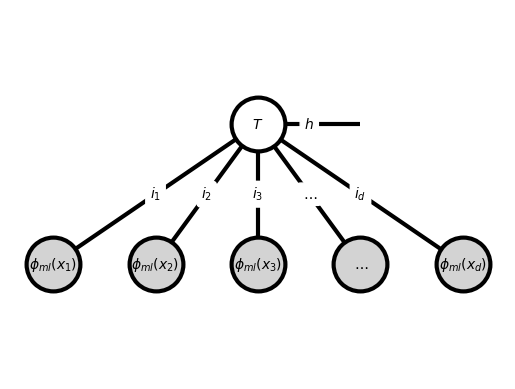
\includegraphics[width=0.7\textwidth]{images/2023-04-20-11-02-45.png}
    \label{fig:full_tensor_model}
\end{figure}
to 
\begin{figure}[hbt!]
    \centering
    \caption{The $Y_{MPS}$ function visualised.}
    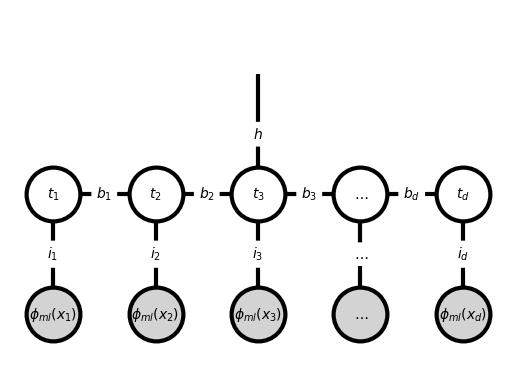
\includegraphics[width=0.7\textwidth]{images/2023-04-20-12-41-57.png}
    \label{fig:mps_tensor_model}
\end{figure}

\subsection{Composition of MPS}
As mentionned before, taking a linear map of  tensor product of the local feature map 
$ x \mapsto \begin{bmatrix} 1 \\ x \end{bmatrix} $ amounts to producing a multilinear function of $\mathbf{x}$.

Since our MPS model can only approximate this function, it means that its expressivity
will be somewhat limited. For example, it could never express the function $f(\mathbf{x}) = x_1x_2^2$, since it is not multilinear. It is however entirely possible that being able to express functions of this type are of great importance when it comes to modeling real world phenomena. There is a simple way to fix this problem which ties nicely with our of goals: distillating knowledge into a student MPS network. Once again, to make things clearer, we will talk about achieving this with the $\Upsilon_{T}$ function first, and talk about the MPS after. Ihe following subsection, we will prove that this composed function can express
any multivariate polynomial function of degree $z$.

\subsubsection{Proof of expressivity}
\begin{definition}[Polynomial function of degree $z$]

    Is a polynomial function $P: R^d \to R$ where every monomial is of the form:
    \[
        cx_1^{k_1} x_2^{k_2}(\dots)x_d^{k_d}
    \]
    where $c$ and the $k$ variables are constants satisfying the condition:
    \[
        \sum_{i=1}^{d}k_i \leq z
    \]
\end{definition}


\begin{theorem}
    For every polynomial function $P$ of degree $z$, there exists tensors $T_1$ and $T_2$ such that
    \[ \Gamma(\mathbf{x}) = \left(\Upsilon_{T_2} \circ \Upsilon_{T_1}\right) (\mathbf{x}), \forall \mathbf{x} \in R^d\]
\end{theorem}

\begin{proof}
Let the tensor $T_1$ be defined such that
\begin{equation}
    \Upsilon_{T_1}(\mathbf{x})
    = 
    \begin{bmatrix}
            x_1   \\
            \vdots  \\
            x_1 \\
            x_2 \\
            \vdots \\
            x_2 \\
            \vdots \\
            x_d  \\
            \vdots  \\
            x_d 
    \end{bmatrix}
\end{equation}
where each of the variables are repeated $z$ times in the vector.

Now, we can perform the vector equivalent of a change of variable by rewriting the vector $\Upsilon_{T_1}(\mathbf{x})$ as a new vector $\bm{\lambda}$ :

\begin{equation} \label{lambda}
    \begin{bmatrix}
        x_1   \\
        \vdots  \\
        x_1 \\
        x_2 \\
        \vdots \\
        x_2 \\
        \vdots \\
        x_d   \\
        \vdots  \\
        x_d
\end{bmatrix}
    =
    \begin{bmatrix}
        \lambda_{1, 1} \\
        \vdots \\
        \lambda_{1, z} \\
        \lambda_{2, 1} \\
        \vdots \\
        \lambda_{2, z} \\
        \vdots \\
        \lambda_{d, 1} \\
        \vdots \\
        \lambda_{d, z} 
    \end{bmatrix}
    = \bm{\lambda}
\end{equation}

Let $\mathbb{P}$ be the space of polynomial functions 
of degree $\leq z$, where the variables are the elements of the vector $\mathbf{x}$. By definition, every monomial of any particular polynomial function $P \in \mathbb{P}$ is of the form
\begin{equation}
    x_{1}^{k_1}x_{2}^{k_2}(\dots)x_{d}^{k_d}
\end{equation}
where the condition $\sum k_i \leq z$ is met. \\
For every set $\{k_1, k_2, (\dots), k_d\}$ meeting this condition,
we can rewrite the monomial as
\begin{equation}
    \left( \prod_{i_1=1}^{k_1}\lambda_{1, i_1} \right)
    \left( \prod_{i_2=1}^{k_2}\lambda_{2, i_2} \right)
    \left( \dots \right)
    \left( \prod_{i_d=1}^{k_d}\lambda_{d, i_d} \right)
\end{equation}
by using the elements of the vector $\lambda$ from equation \eqref{lambda}.

However, we can clearly see that this term is a multilinear 
monomial of the variables in $\lambda$. This implies that
$Y_{T_2}(\bm{\lambda})$ can express any polynomial function of degree $z$ by setting $T_2$ properly.





\end{proof}
It seems we have just solved our problem. Since
\[
    \lim_{B\to\infty}
    \left(\Upsilon_{MPS_2} \circ \Upsilon_{MPS_1}\right) (\mathbf{x})
    =
    \left(\Upsilon_{T_2} \circ \Upsilon_{T_1}\right) (\mathbf{x})
\]
where $B$ is the bond dimension of the two $MPS$.
We only proved that this is only true if the output dimension of $MPS_1$ is of dimension $\geq dz$, where $d$ is the dimension of the input vector $\mathbf{x}$ and $z$ is the degree of the Polynomial. This is fine, because this is not exponential in $d$. However, the model might not require this amount of expressivity. If the output dimension is less then $zd$, it can learn to \emph{choose} which variables of the input vectors deserve more complexity. This is interesting.


TODO mention the 2-MPS name.
2 par 2 par 2 pr 2
bon dimension parfaite a 


\section{Methodology}
The experiments done for the projet were programmed using Python and the wonderful deep learning library Pytorch, created by Meta.
Unfortunately, Pytorch does not provide any tools to train and build Tensor Networks. 
Luckily for us, Jacob Miller, created a library \cite{torchmps} built on top of Pytorch that provides the tools to build and train MPS Tensor Networks. The library is extremely easy while providing a lot of options.

\subsection{The Task}
All of our models were trained to perform a classification task on the popular MNIST Dataset. This dataset contains several handwritten digits and the classes are the integers from $0$ to $9$. In order to be able to make more experiments, we only took a subset of $2000$ training examples and $500$ test examples. These remained invariant through the training of each model. In other words, we kept the same subsets during the training of the different models in our experiments.

\subsection{Bad Teacher, Good Teacher}
In our experiments, we use two teachers to train the student (MPS): one who performed poorly and one who performed goodly.
The bad teacher is a simple Multi Layer Perceptron of $4$ hidden layers of $70$ hidden neurons each with the $ReLU$ activation function.  The good teacher was a ConvNet (CNN) with a very basic architecture.


\subsection{Distillation Procedure}
For the distillation, we only used the outputs of the teacher to train the student. In other words, the student never had direct access to the labels during the training. The Distillation occured in two steps. \\ On the first step, the student was trained on the outputs of the teacher with inputs being examples from the training set with adde Gaussian noise for $25$ epochs. The added Gaussian noise had a mean $\mu=0$ and a variance $\sigma^2=0.2$. \\ On the second step, the student was trained on the outputs of the teacher with inputs being direct examples from the training for $25$ epochs.
TODO: mention this is not true for the bad teacher

\subsection{Hyperparameters of the MPS}
\begin{enumerate}
    \item Learning Rate $= 1e-4$
    \item Regularisation $= 0$
    \item Loss Function: Cross Entropy
    \item Bond Dimensions: Varies with the experiment
\end{enumerate}

\subsection{The Experiments}
Our first experiment was to train the MPS with different bond dimensions (10, 20, 40 and 80). The accuracy of these models on the test dataset is our baseline. This experiment was repeated $20$ times for each bond dimension. Our goal was to get a better idea with mean and variance.

The next series was similar to the last one, but instead of training the MPS on the $labels$, we trained it on distribution given by the bad teacher using the Kullback-Leibner divergence loss.

The last series of experiment is the same as the last one, but with the good teacher.

\subsection{Double MPS}
You might be wondering why we have not mentionned the double-MPS yet. Well it is because it appears that the backpropagtion learning algorithm had numerical problems to train the baseline of the double MPS. Since we could not create a baseline, we were suggested to concentrate our ressources to the other experiments. Reasons for this issue will be mentionned in the \emph{Analysis} section. 





TODO: mention custom feature map in forked code


\section{Results}
\paragraph{Accuracy of the bad teacher}
The good teacher, which is a ConvNet, had a classification accuracy of $0.54$ on the $500$ examples of the test set.

\paragraph{Accuracy of the good teacher}
The good teacher, which is a ConvNet, had a classification accuracy of $0.97$ on the $500$ examples of the test set. \\

\subsection{Final Accuracys}
In the table below, you will find the final classification accuracy of every model on the test dataset. As mentionned in the methodology, each of these experiments was repeated 20 times in order to get the standard deviation. \\

\begin{center}
\begin{tabular}{ | c | c | c | c | }
\hline 
Bond Dimensions & MPS & FC to MPS & CNN to MPS \\ 
\hline
10 & $0.897 \pm 1.16 \times 10^{-2}$  & $0.541 \pm 9.75 \times 10^{-3}$ & $0.906 \pm 9.23 \times 10^{-3}$ \\
20 & $0.911 \pm 1.14 \times 10^{-2}$ & $0.550 \pm 9.65 \times 10^{-3}$ & $0.924 \pm 8.23 \times 10^{-3}$ \\ 
40 & $0.914 \pm 9.03 \times 10^{-3}$ & $0.556 \pm 7.74 \times 10^{-3}$ & $0.941 \pm 6.62 \times 10^{-3}$ \\
80 & $0.916 \pm 1.77 \times 10^{-2}$ & $$ & $0.944 \pm 8.58 \times 10^{-3}$ \\
\hline
\end{tabular}
\end{center}

\subsection{Accuracy during training}
We \emph{figured} it would be of use to include \emph{figures} which show the accuracy and the standard devitations at each epoch during the training.
\begin{figure}[H]
    \centering
    \caption{}
    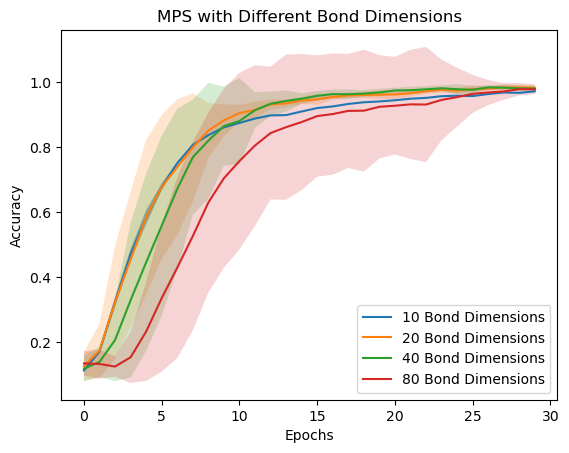
\includegraphics[width=0.8\textwidth]{images/2023-04-21-18-13-34.png}
    \label{fig:MPS}
\end{figure}

\begin{figure}[H]
    \centering
    \caption{}
    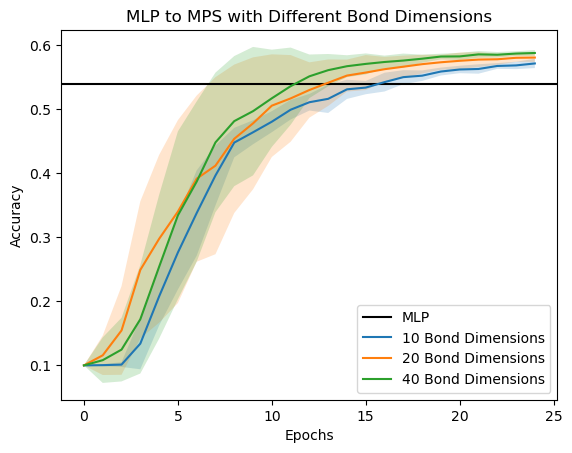
\includegraphics[width=0.8\textwidth]{images/images/2023-04-21-18-13-34.png.png}
    \label{fig:MLP_to_MPS}
\end{figure}

\begin{figure}[H]
    \centering
    \caption{}
    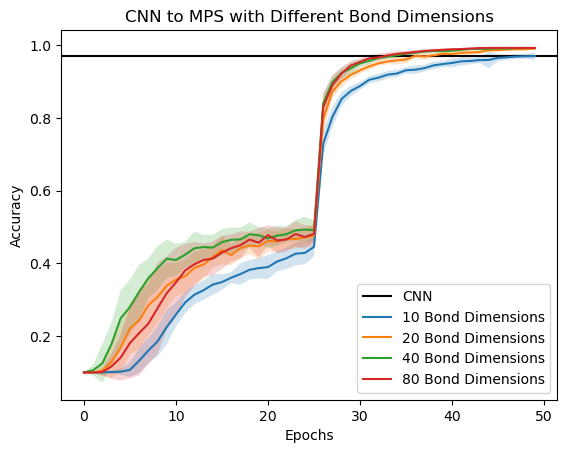
\includegraphics[width=0.8\textwidth]{images/2023-04-21-18-13-15.png}
    \label{fig:CNN_to_MPS}
\end{figure}



\subsection{Double MPS}
The Double MPS was able to get an accuracy of $0.524$ with the bad teacher.

\section{Analysis}

\subsection{Bad Teacher : MLP to MPS}
\begin{figure}[hbt!]  \label{fig:function_space}
    \centering
    \caption{Illustration of bias and variance in divergence from the goal function.}
    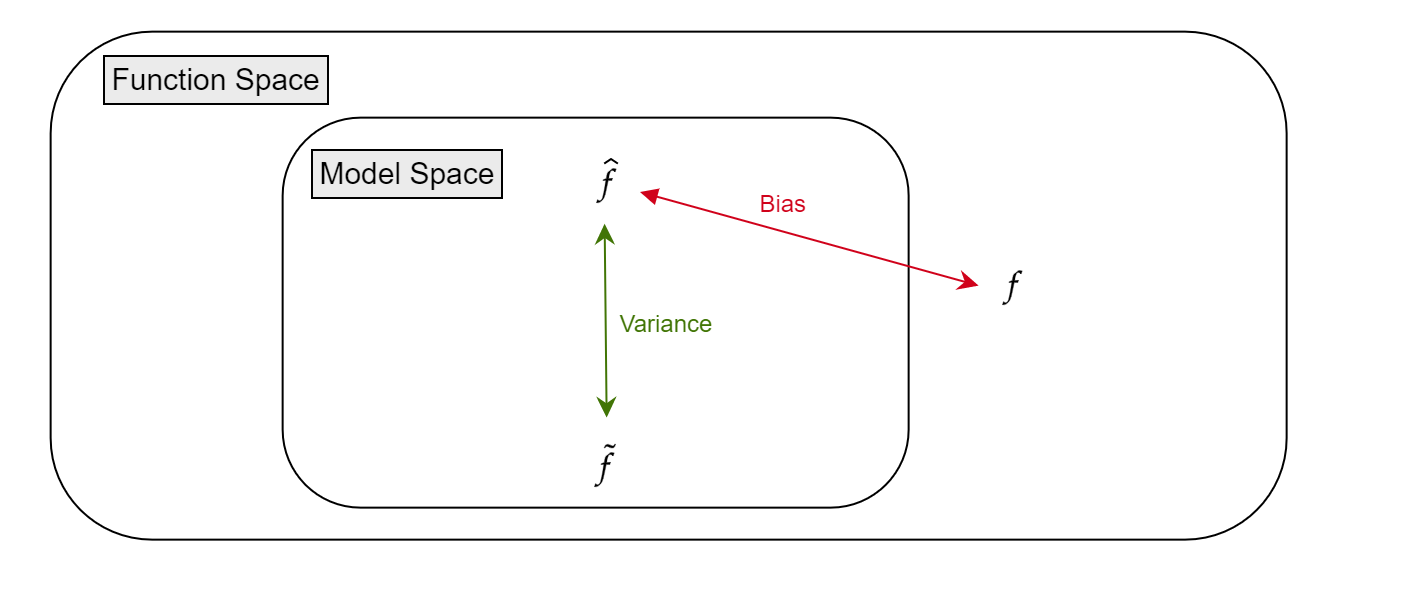
\includegraphics[width=0.8\textwidth]{images/2023-04-21-16-47-59.png}
    \floatfoot{Here, $f$ represents the goal function (the function we want to learn), $\hat{f}$ is the closest function to $f$ that our model can express and $\tilde{f}$ represents the function we can expect to obtain during training.}
\end{figure}

The first interesting result is that the MPS trained by the bad teacher generalises better than it to unseen data. One explanation for this is that their is less of a bias of the MPS towards the function we were trying to learn than for the MLP. This is suprising, considering that MLP's are known to have a really low bias. The Figure \ref{function_space} might help us visualise this. Here, the distance from the goal function $f$ is caused by the variance and the bias. In our experiments, there was no variance in the examples. The only variance was in the initialisation of the models. This leads us to believe that the real cause of the disparity has more to do with the bias. To confirm this, it would be a good idea to repeat the experiment multiple times and retrain the bad model each time to see if the MPS keeps getting better scores after distillation.

\subsection{Good Teacher : CNN to MPS}
As you can see, the distilled MPS manages to perform better than the MPS on it's own. Amazingly, this is true for every bond dimension in our experiments (10, 20, 40 and 80). This means that on the same limited subset, we can make a MPS generalise better on a goal function with the help of a CNN model. This finding is, as of now, purely of theoretical use. This is due to the fact that the simple CNN we trained, which performs better than the MPS at every bond dimension, as way less parameters and takes less times to compute. As mentionned in the methodology,
TODO: mention distillation with gauss order importance



\section{Conclusion}



\subsection{Further Exploration}
TODO talk about the patch MPS
TODO talk about capturing locality in the mappings
TODO talk about capturing locality in general with tensors

\printbibliography

\end{document}




































Person 1: *waiving vigorously
    HELLO CAN YOU SEE ME!
    HEYYY! 

Person 2:
    For the last time, they can't see you... 
    YOU'RE OUTSIDE THE DOCUMENT DELIMITERS!

Person 1: 
    I feel so alone... 

Person 2: 
    Bro I'm here...